Since source code is listed as one of the deliverables in the assignment text, I show you here the source code of my python implementation of the linear regression algorithm, as it is described in the Data Mining Lecture Notes by Christian Igel: 

\begin{verbatim}
import scipy as scp

def linear_regression(x, y) :
    
    if (x.ndim == 1) : x = scp.matrix(x).T
    else : x = scp.matrix(x)
    y = scp.matrix(y).T
    
    
    ones_column = scp.tile([1], (x.shape[0], 1))
    x = scp.concatenate((x, ones_column), axis=1)
    
    w = (((((x.T * x).I) * x.T))* y ).A
    
    b = w[-1,0]
    w = w[0:-1].flatten()
    
    predict = lambda new : scp.dot(w, new) + b
    
    return {'hyp' : predict, 
            'est_params' : {'weigths': w, 
                            'bias': b}}
\end{verbatim}

The implementation uses the scipy library to take care of the linear algebra. As input it takes a scipy 2d-array as x (the sample) and a scipy 1d-array as y (the labels). As output it gives a dictionary containing 1) the linear model, which minimizes the squared error between the models predictions and the actual labels, and 2) the weight and bias parameters of the model. When I run this implementation on the Danwood data, I get the weight parameter 9.489 and the bias parameter -10.427. This means that my resulting model $h$ looks like:

\begin{align}
h(x) = 9.489x - 10.427
\end{align}

When I plot this model against the actual data, I get the following plot:

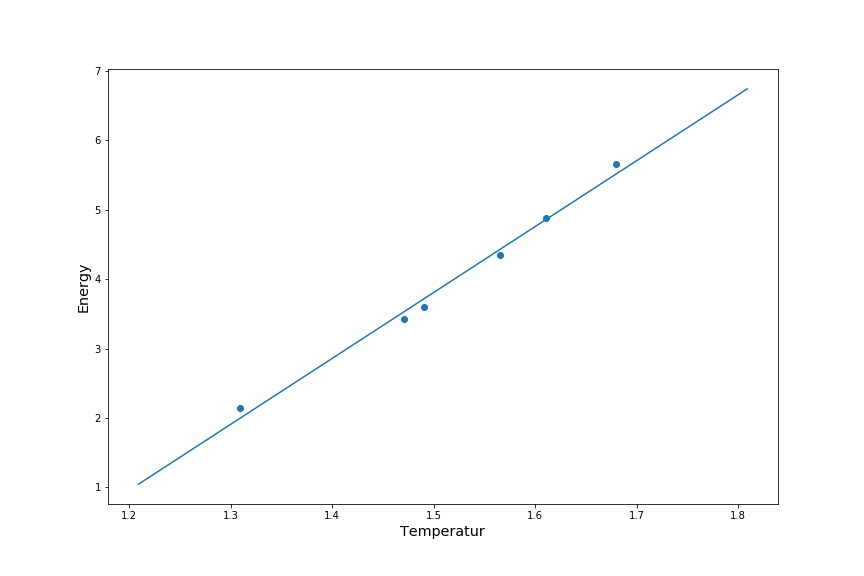
\includegraphics[scale = 0.45]{linear_regression/reg_plot_1.jpg}

The mean squared error of this model is 0.012. The variance of y (the energy measurements) is 1.269. The quotient of the mean squared error of the model over variance of y is 0.009. There are multiple ways to interpret this number in the context of linear regression. One way is to say that it is a measure of the how much smaller the error is, when we choose all linear functions as our model space instead of just constant functions (since the mean of y would be the squared error minimizer in the space of all constant models, and therefore the variance of y would be the mse of the chosen model in this space). In this interpretation it becomes clear that the quotient cannot be larger than 1, since the constant models are a subclass of the linear models. This also shows us that just because the quotient is a little smaller than 1, this does not mean that we have made a good decision by choosing all linear functions as our model space. It is not good to choose a much more complex model space, if we just get a small error reduction from it (especially in our current set up of linear regression, where we have no distinction between training and test set!). However, with the Danwood data we get approximately a reduction of factor 100, so it might be a good idea to model the data with linear instead of just constant functions. This is also quite obvious from just looking at the data (the orange line is the best constant model):

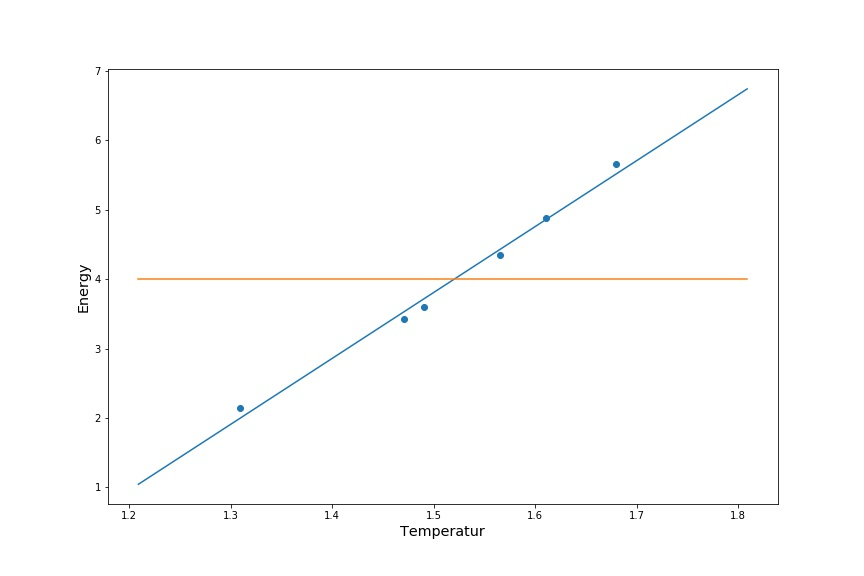
\includegraphics[scale = 0.45]{linear_regression/reg_plot_2.jpg}

